%
% buergiausschnitt.tex -- template for standalon tikz images
%
% (c) 2021 Prof Dr Andreas Müller, OST Ostschweizer Fachhochschule
%
\documentclass[tikz]{standalone}
\usepackage{amsmath}
\usepackage{times}
\usepackage{txfonts}
\usepackage{pgfplots}
\usepackage{csvsimple}
\usetikzlibrary{arrows,intersections,math}
\begin{document}
\def\skala{1}
\begin{tikzpicture}[>=latex,thick,scale=\skala]

\def\w{7.5}
\def\h{10}

\begin{scope}
\clip (-7.4,-10.4) rectangle (7.9,12.1);
\node at (0,0) {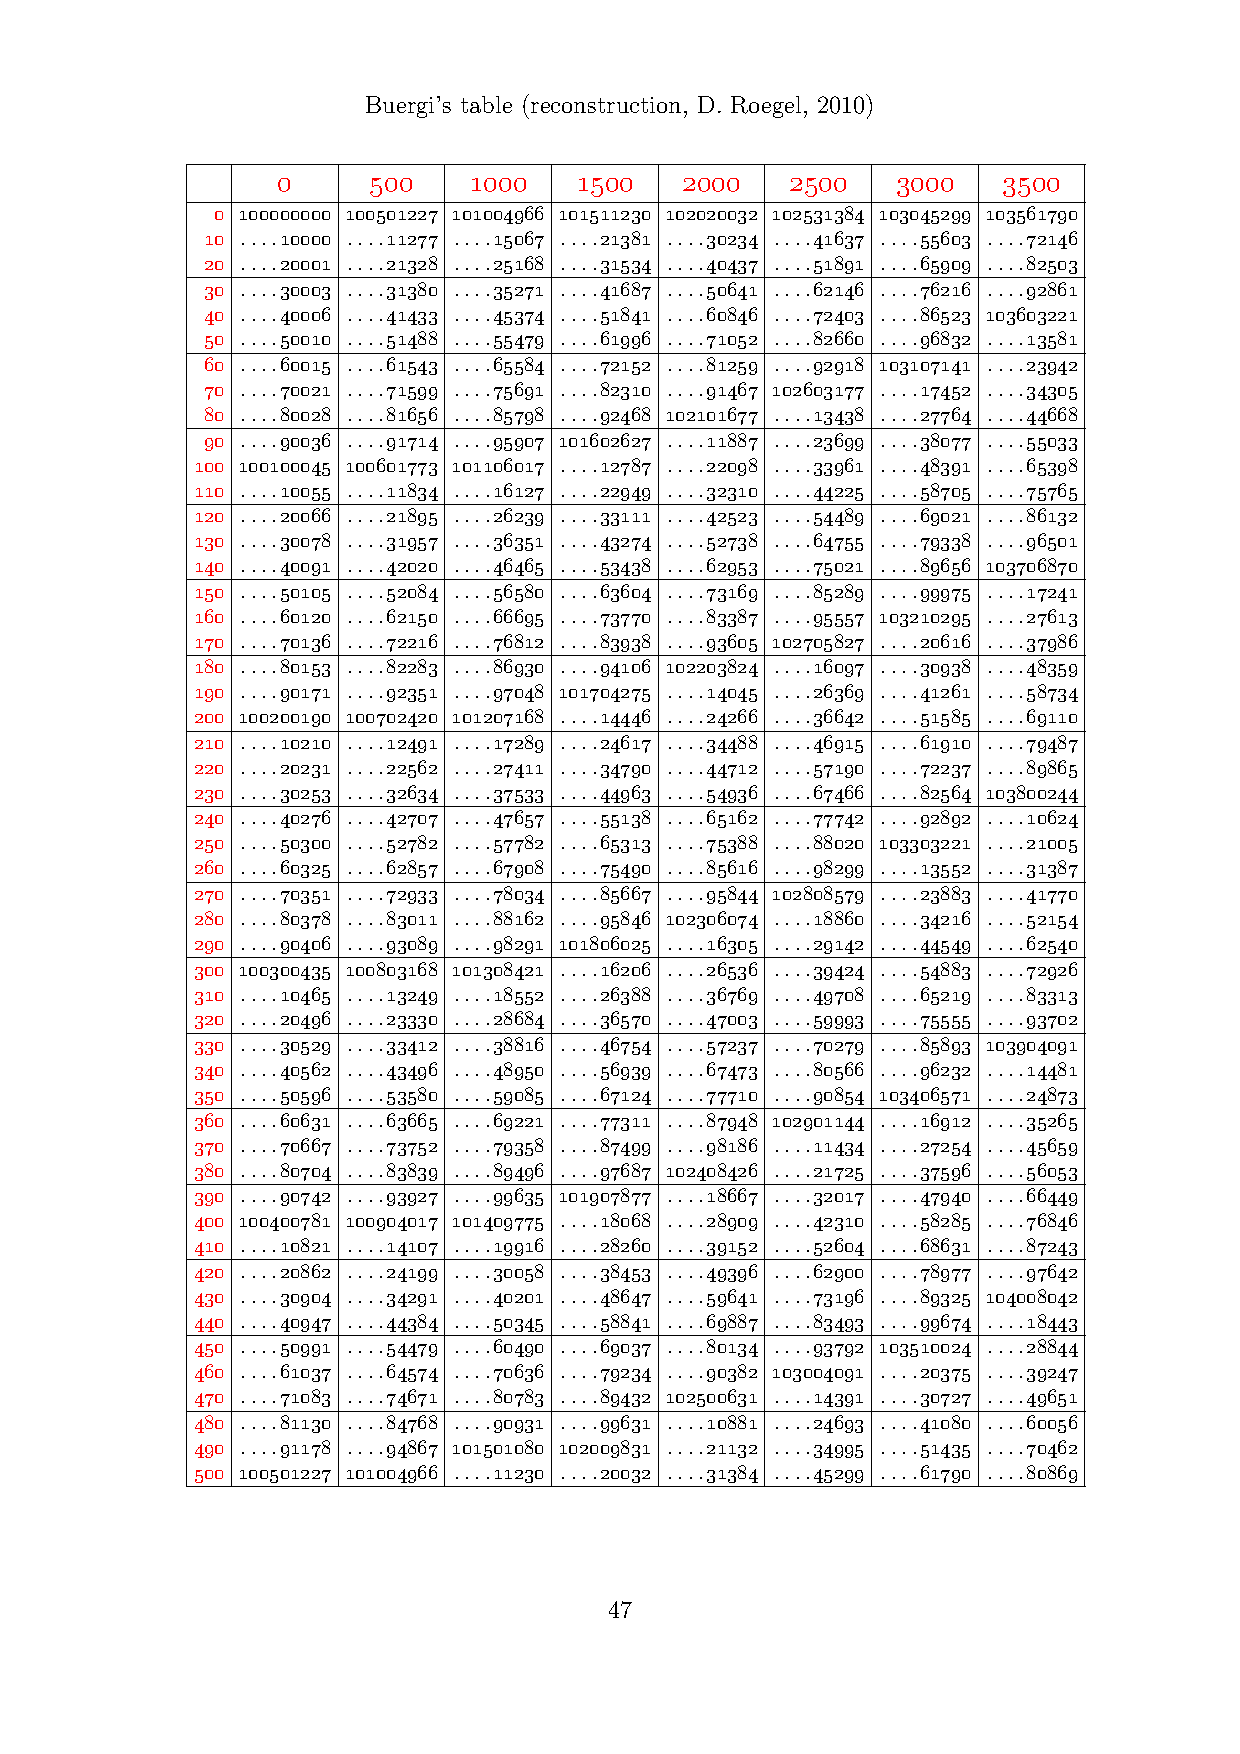
\includegraphics{buergi1.pdf}};
\end{scope}

\end{tikzpicture}
\end{document}

